% $Header$
 
\documentclass[trans]{beamer}

\mode<presentation>
{
  \usetheme{CambridgeUS}
  \setbeamercovered{transparent}
}

\usepackage[english]{babel}
\usepackage[latin1]{inputenc}
\usepackage{times}
\usepackage[T1]{fontenc}

% === dcolumn package ===
\usepackage{dcolumn}
\newcolumntype{.}{D{.}{.}{-1}}
\newcolumntype{d}[1]{D{.}{.}{#1}}

% === new commands ===
\newcommand\ud{\mathrm{d}}
\newcommand\dist{\buildrel\rm d\over\sim}
\newcommand\ind{\stackrel{\rm indep.}{\sim}}
\newcommand\iid{\stackrel{\rm i.i.d.}{\sim}}
\newcommand\logit{{\rm logit}}
\renewcommand\r{\right}
\renewcommand\l{\left}
\newcommand\cA{\mathcal{A}}
\newcommand\cJ{\mathcal{J}}

\newcommand\independent{\protect\mathpalette{\protect\independenT}{\perp}}
\def\independenT#1#2{\mathrel{\rlap{$#1#2$}\mkern2mu{#1#2}}}

%%%%%%%%%%%%%%%%%%%%%%%%%%%%%%%%%%%%%%%%%%%%%%%%%%%%%%%%%%%%%%%%%%%%%%

\title[The Balance Test Fallacy]{The Balance Test Fallacy in Matching
  Methods for Causal Inference}

\author{Kosuke Imai}

\institute[Princeton University]{
  Department of Politics\\
  Princeton University \\
  \vskip .1in
  Joint work with\\
  {\bf Gary King} \\ Department of Government, Harvard University \\
  \vskip .05in {\bf Elizabeth A. Stuart} \\ Bloomberg School of Public
  Health, Johns Hopkins University }

\date[]{August 31, 2006}

\subject{Balance Tests in Matching Methods}


% If you wish to uncover everything in a step-wise fashion, uncomment
% the following command: 
\beamerdefaultoverlayspecification{<+->}

\begin{document}

\begin{frame}
  \titlepage
\end{frame}


%%%%%%%%%%%%%%%%%%%%%%%%%%%%%%%%%%%%%%%%%%%%%%%%%%%%%%%%%%%%%%%%

\section{Introduction}

\begin{frame}
  \frametitle{What is Matching? How does It Help Us?}
\begin{itemize}
\item A popular method for causal inference across academic fields.
  
\item Matching as a nonparametric preprocessing procedure to improve
  parametric analysis by reducing model dependence (Ho, Imai, King and
  Stuart, 2006).
  
  \begin{itemize}
  \item Assumption: ``no omitted variable.''
  \item Goal: eliminate the (in-sample) relationship between the
    observed covariates $X$ and the treatment variable $T$ by
    dropping, repeating, and/or grouping observations.
  \item Best case: the matched data satisfy the perfect balance,
    $$\tilde p(X\mid T=1) \; = \; \tilde p(X \mid T=0),$$
    which
    implies no need for subsequent adjustments for $X$.
  \item In practice: adjust for the remaining imbalance via the same
  parametric methods as would have been applied if matching had not
  been conducted.
 \end{itemize}
 
\item A number of matching algorithms are being developed.
\end{itemize}
 \end{frame}

%%%%%%%%%%%%%%%%%%%%%%%%%%%%%%%%%%%%%%%%%%%%%%%%%%%%%%%%%%%%%%%% 

\section{Problems with Hypothesis Tests as Stopping Rules}

\begin{frame}
  \frametitle{Assessing the Balance in Matching Methods}

\begin{itemize}
\item The success of any matching method depends on the resulting
  covariate balance.
  
\item How should one assess the balance of matched data?
  \begin{itemize}
    
  \item Ideally, one would like to compare the joint distribution of
    all covariates for the matched treatment and control groups.
    
  \item In practice, this is impossible when $X$ is high-dimensional.
  \end{itemize}

\item Standard practice: use of balance test
  \begin{itemize}
  \item $t$ test for difference in means for each variable of $X$.
  \item other test statistics such as $\chi^2$, $F$,
    Kolmogorov-Smirnov tests are also used.
  \item statistically insignificant test statistics are used as a
    justification for the adequacy of the chosen matching method and
    a stopping rule for maximizing balance.
  \item the practice is widespread across disciplines (economics,
    education, management science, medicine, public health,
    psychology, and statistics).
  \end{itemize}

\end{itemize}
\end{frame}

%%%%%%%%%%%%%%%%%%%%%%%%%%%%%%%%%%%%%%%%%%%%%%%%%%%%%%%%%%%%%%%% 

\begin{frame}
  \frametitle{An Illustration of Balance Test Fallacy}

\begin{minipage}[l]{1.75in}
  \begin{itemize}
  \item School Dropout Demonstration Assistance Program.
  \item Treatment: school ``restructuring'' programs.
  \item Outcome: dropout rates.
  \item We look at the baseline math test score.
  \item ``Silly'' matching algorithm: randomly selects control units
    to discard.
  \end{itemize}
\end{minipage}
\begin{minipage}[l]{1in}
  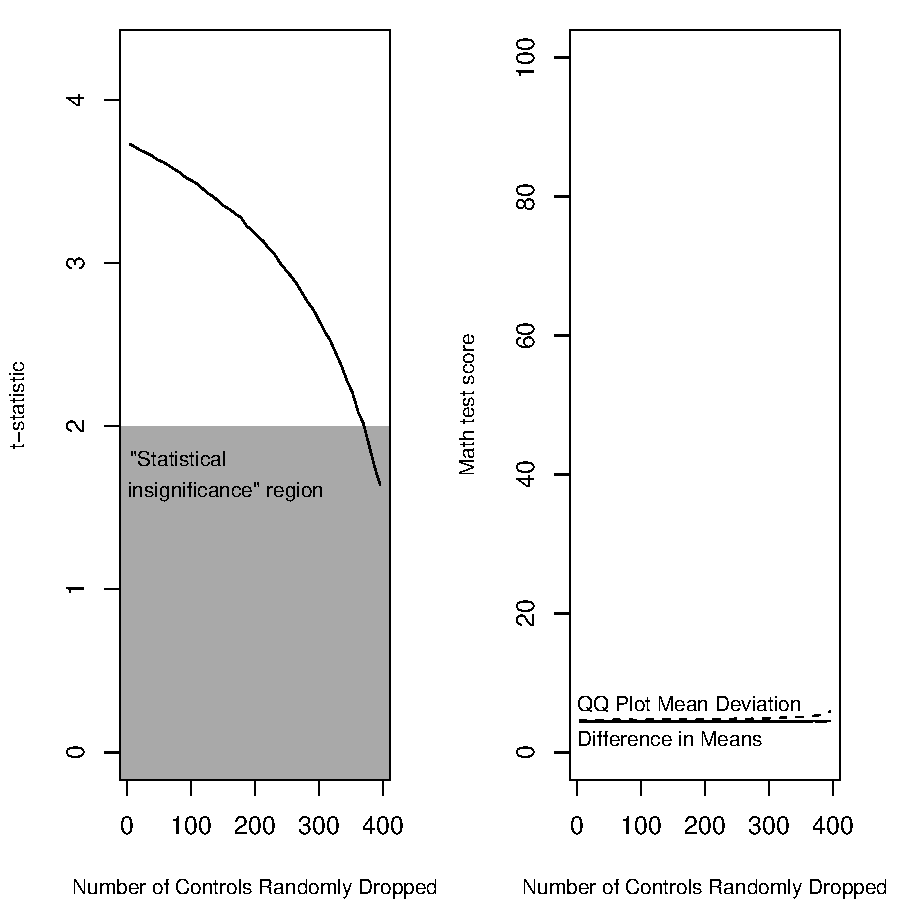
\includegraphics[scale=0.5]{figs/TStatPlotR0MATH}
\end{minipage}

\end{frame}

\begin{frame}
  \frametitle{Problems with Hypothesis Tests as Stopping Rules}

  \begin{enumerate}
  \item[1] Balance test is a function of both balance and statistical
    power: the more observations dropped, the less power the tests
    have to detect imbalance in observed covariates.
  \item[2] $t$-test is affected by factors other than balance,
    $$\frac{\sqrt{n_m}(\overline{X}_{mt}-\overline{X}_{mc})}
    {\sqrt{\frac{s^2_{mt}}{r_m} + \frac{s^2_{mc}}{1-r_m}}}$$
    \begin{itemize}
    \item $\overline{X}_{mt}$ and $\overline{X}_{mc}$ are the sample
      means.
    \item $s^2_{mt}$ and $s^2_{mc}$ are the sample variances.
     \item $n_m$ is the total number of remaining observations.
     \item $r_m$ is the ratio of remaining treated units to the total
       number of remaining observations.
     \end{itemize}
   \end{enumerate}
\end{frame}

\begin{frame}
  \frametitle{Problems with Hypothesis Tests as Stopping Rules}

  \begin{enumerate}
   \item[3] In theory, a balance is a characteristic of the (matched)
     sample rather than of some hypothetical population, and hence
     hypothesis tests are irrelevant.
     \begin{itemize}
     \item Virtually all methods of adjustments condition on the
       observed values of $X$.
     \item Even in randomized experiments, matched-pair or randomized
       blocks designs are {\it always} preferable to simple
       randomization.
     \end{itemize}

   \item[4] Even a small imbalance can greatly affect the resulting
   causal estimates.
   \begin{itemize}
   \item Linear regression: $E(Y \mid T, X) = \theta + T\beta +
     X\gamma$. 
   \item Bias: $E(\hat{\beta} - \beta \mid T, X) = G \gamma$ where
     $\hat{\beta}$ is the difference in means estimator and $G$
     contains vector of coefficients from regression of each of the
     covariates in $X$ on a constant and $T$.
   \item A similar argument has been made in the context of randomized
     experiments (e.g., Altman 1985; Senn, 1994; Pocock et al., 2002).
   \end{itemize}
   
   \end{enumerate}

\end{frame}

%%%%%%%%%%%%%%%%%%%%%%%%%%%%%%%%%%%%%%%%%%%%%%%%%%%%%%%%%%%%%%%% 

\section{Concluding Remarks}
\begin{frame}
  \frametitle{Concluding Remarks}

\begin{itemize}
\item Balance should be assessed by comparing the observed covariate
  differences between the treated and control groups.

\item These observed differences should be minimized without limit. 
  
\item A variety of balance measures can be considered: (standardized)
  differences in sample means, ratios of sample variances, higher
  order moments, statistics based on quantile-quantile plots etc.
  
\item In published articles, reported small $p$-values and large
  $t$-statistics should cause readers to worry about balance, whereas
  the reverse would not suggest any level of comfort.
  
\item In observational studies, remaining imbalance, however small,
  could be due to chance or to systematic differences.
\end{itemize}

\end{frame}

\end{document}


